\chapter{Momentová okrajová podmínka ve 2D}\label{priloha A}
V sekci \ref{moment based bc} je obecně popsána momentová okrajová podmínka, kterou lze v rámci LBM použít. Pro úplnost uvedeme konkrétní případ použití této okrajové podmínky v rámci použitého rychlostního modelu D2Q9. Jak bylo zmíněno v sekci \ref{moment based bc}, vztahy pro výpočet neznámých distribučních funkcí musí být použity pro 4 různé strany obdélníkové oblasti a 4 zbývající navzájem různé rohy této oblasti $ \Omega $. Různé části hranice výpočetní oblasti budeme značit podle obr. \ref{fig:oblast pro MBBC}.

\begin{figure}[H]
	\vspace{4mm}
	\centering
	\includegraphics[width=0.85\textwidth]{Images/oblastBC.pdf}
	\vspace{4mm}
	\caption{Schematické znázornění označení částí výpočetní oblasti $ \Omega $. Označením jsou rozlišeny jednotlivé strany, resp. rohy výpočetní oblasti.}  
	\label{fig:oblast pro MBBC}
	\vspace{1.8mm}
\end{figure}

Dále pro každou z částí hranice výpočetní oblasti uvedeme, které momenty a s jakými koeficienty byly zvoleny pro vyjádření neznámých distribučních funkcí. Dále vždy uvedeme explicitní vyjádření výpočtu $ \rho $ pomocí distribučních funkcí a složek rychlosti. Podotkněme, že v případě, kdy by byla na jedné z částí hranice zadaná hodnota $ \rho $ a měla být vyjádřena neznámá rychlost, lze výpočetní vztah jednoduše vyjádřit z uvedeného vztahu pro výpočet $ \rho $.

Jak bylo zmíněno v sekci \ref{moment based bc}, pro implementaci momentové okrajové podmínky pro model D2Q9 byl využit generátor vytvořený Ing. Pavlem Eichlerem, viz \cite{PE}. Dále uvedené tvary momentové okrajové podmínky pro jednotlivé části hranice jsou pak také výsledkem zmíněného generátoru.

\newpage
%W
\section*{Část W}
¨
\begin{table}[!h]
	\centering
	\begin{tabular}{c l l l}
		\toprule
		\# & Momenty & Neznámé kombinace $f$ & Zvolené\\
		\midrule
		\multirow{ 1}{*}{$1$} & \multirow{ 1}{*}{$m_\bb{0,0}, m_\bb{1,0}, m_\bb{2,0}$} & $f_1+f_8+f_5$ & \multirow{ 1}{*}{$m_\bb{1,0}$}\\ 
		\midrule
		\multirow{ 1}{*}{$2$} & \multirow{ 1}{*}{$m_\bb{0,1}, m_\bb{1,1}, m_\bb{2,1}$} & $-f_8+f_5$ & \multirow{ 1}{*}{$m_\bb{0,1}$}\\ 
		\midrule
		\multirow{ 1}{*}{$3$} & \multirow{ 1}{*}{$m_\bb{0,2}, m_\bb{1,2}, m_\bb{2,2}$} & $f_8+f_5$ & \multirow{ 1}{*}{$m_\bb{0,2}$}\\ 
		\bottomrule
\end{tabular}\end{table}

\begin{table}[!h]
	\centering
	\begin{tabular}{l l}
		\toprule
		Neznámá & Řešení\\
		\midrule
		$\rho$ & $-\frac{2 f_6+2 f_3+f_0+2 f_7+f_4+f_2}{-1+u_1}$ \\ 
		\bottomrule
\end{tabular}\end{table}

\begin{subequations}
	\begin{equation}
	\begin{pmatrix}f_1 \\ f_5 \\ f_8 \end{pmatrix} = \mathbb{A}_f
	\begin{pmatrix}f_0 \\ f_2 \\ f_3 \\ f_4 \\ f_6 \\ f_7 \end{pmatrix} + \mathbb{A}_m \begin{pmatrix}
	m_\bb{1,0} \\ m_\bb{0,1} \\ m_\bb{0,2}\end{pmatrix},
	\end{equation}
	kde 
	 
	\begin{equation}
	\mathbb{A}_f = \begin{pmatrix}0 &	1 &	1 &	1 &	2 &	2\\
	0 &	-1 &	0 &	0 &	-1 &	0\\
	0 &	0 &	0 &	-1 &	0 &	-1
	\end{pmatrix},
	\end{equation}
	\normalsize
	a 
	  
	\begin{equation}
	\mathbb{A}_m = \begin{pmatrix}1 &	0 &	-1\\
	0 &	\frac{1}{2} &	\frac{1}{2}\\
	0 &	-\frac{1}{2} &	\frac{1}{2}
	\end{pmatrix}.
	\end{equation}
	\normalsize
\end{subequations}
\newpage

%WN
\section*{Část WN}
\noindent S použitím generátoru momentové okrajové podmínky z \cite{PE} platí:\\

\begin{table}[!h]
	\centering
	\begin{tabular}{c l l l}
		\toprule
		\# & Momenty & Neznámé kombinace $f$ & Zvolené\\
		\midrule
		\multirow{ 1}{*}{$1$} & \multirow{ 1}{*}{$m_\bb{0,0}$} & $f_7+f_4+f_1+f_8+f_5$ & \multirow{ 1}{*}{--}\\ 
		\midrule
		\multirow{ 1}{*}{$2$} & \multirow{ 1}{*}{$m_\bb{1,0}$} & $-f_7+f_1+f_8+f_5$ & \multirow{ 1}{*}{$m_\bb{1,0}$}\\ 
		\midrule
		\multirow{ 1}{*}{$3$} & \multirow{ 1}{*}{$m_\bb{0,1}$} & $-f_7-f_4-f_8+f_5$ & \multirow{ 1}{*}{$m_\bb{0,1}$}\\ 
		\midrule
		\multirow{ 1}{*}{$4$} & \multirow{ 1}{*}{$m_\bb{1,1}$} & $f_7-f_8+f_5$ & \multirow{ 1}{*}{$m_\bb{1,1}$}\\ 
		\midrule
		\multirow{ 1}{*}{$5$} & \multirow{ 1}{*}{$m_\bb{2,0}$} & $f_7+f_1+f_8+f_5$ & \multirow{ 1}{*}{$m_\bb{2,0}$}\\ 
		\midrule
		\multirow{ 1}{*}{$6$} & \multirow{ 1}{*}{$m_\bb{0,2}$} & $f_7+f_4+f_8+f_5$ & \multirow{ 1}{*}{$m_\bb{0,2}$}\\ 
		\midrule
		\multirow{ 1}{*}{$7$} & \multirow{ 1}{*}{$m_\bb{2,1}$} & $-f_7-f_8+f_5$ & \multirow{ 1}{*}{--}\\ 
		\midrule
		\multirow{ 1}{*}{$8$} & \multirow{ 1}{*}{$m_\bb{1,2}$} & $-f_7+f_8+f_5$ & \multirow{ 1}{*}{--}\\ 
		\midrule
		\multirow{ 1}{*}{$9$} & \multirow{ 1}{*}{$m_\bb{2,2}$} & $f_7+f_8+f_5$ & \multirow{ 1}{*}{--}\\ 
		\bottomrule
\end{tabular}\end{table}

\begin{table}[!h]
	\centering
	\begin{tabular}{l l}
		\toprule
		Neznámá & Řešení\\
		\midrule
		$\rho$ & $\frac{2 f_2+4 f_6+2 f_3+f_0}{1+u_2- {(1+u_2)} u_1}$ \\ 
		\bottomrule
\end{tabular}\end{table}

\begin{subequations}
	\begin{equation}
	\begin{pmatrix}f_1 \\ f_4 \\ f_5 \\ f_7 \\ f_8 \end{pmatrix} = \mathbb{A}_f
	\begin{pmatrix}f_0 \\ f_2 \\ f_3 \\ f_6 \end{pmatrix} + \mathbb{A}_m \begin{pmatrix}
	m_\bb{1,0} \\ m_\bb{0,1} \\ m_\bb{1,1} \\ m_\bb{2,0} \\ m_\bb{0,2}\end{pmatrix},
	\end{equation}
	kde 
	 
	\begin{equation}
	\mathbb{A}_f = \begin{pmatrix}0 &	2 &	1 &	4\\
	0 &	1 &	2 &	4\\
	0 &	-1 &	0 &	-1\\
	0 &	0 &	-1 &	-1\\
	0 &	-1 &	-1 &	-3
	\end{pmatrix},
	\end{equation}
	\normalsize
	a 
	  
	\begin{equation}
	\mathbb{A}_m = \begin{pmatrix}1 &	-1 &	1 &	0 &	-1\\
	1 &	-1 &	1 &	-1 &	0\\
	0 &	\frac{1}{2} &	0 &	0 &	\frac{1}{2}\\
	-\frac{1}{2} &	0 &	0 &	\frac{1}{2} &	0\\
	-\frac{1}{2} &	\frac{1}{2} &	-1 &	\frac{1}{2} &	\frac{1}{2}
	\end{pmatrix}.
	\end{equation}
	\normalsize
\end{subequations}
\newpage
%WS
\section*{Část WS}
\noindent S použitím generátoru momentové okrajové podmínky z \cite{PE} platí:\\

\begin{table}[!h]
	\centering
	\begin{tabular}{c l l l}
		\toprule
		\# & Momenty & Neznámé kombinace $f$ & Zvolené\\
		\midrule
		\multirow{ 1}{*}{$1$} & \multirow{ 1}{*}{$m_\bb{0,0}$} & $f_6+f_1+f_8+f_5+f_2$ & \multirow{ 1}{*}{--}\\ 
		\midrule
		\multirow{ 1}{*}{$2$} & \multirow{ 1}{*}{$m_\bb{1,0}$} & $-f_6+f_1+f_8+f_5$ & \multirow{ 1}{*}{$m_\bb{1,0}$}\\ 
		\midrule
		\multirow{ 1}{*}{$3$} & \multirow{ 1}{*}{$m_\bb{0,1}$} & $f_6-f_8+f_5+f_2$ & \multirow{ 1}{*}{$m_\bb{0,1}$}\\ 
		\midrule
		\multirow{ 1}{*}{$4$} & \multirow{ 1}{*}{$m_\bb{1,1}$} & $-f_6-f_8+f_5$ & \multirow{ 1}{*}{$m_\bb{1,1}$}\\ 
		\midrule
		\multirow{ 1}{*}{$5$} & \multirow{ 1}{*}{$m_\bb{2,0}$} & $f_6+f_1+f_8+f_5$ & \multirow{ 1}{*}{$m_\bb{2,0}$}\\ 
		\midrule
		\multirow{ 1}{*}{$6$} & \multirow{ 1}{*}{$m_\bb{0,2}$} & $f_6+f_8+f_5+f_2$ & \multirow{ 1}{*}{$m_\bb{0,2}$}\\ 
		\midrule
		\multirow{ 1}{*}{$7$} & \multirow{ 1}{*}{$m_\bb{2,1}$} & $f_6-f_8+f_5$ & \multirow{ 1}{*}{--}\\ 
		\midrule
		\multirow{ 1}{*}{$8$} & \multirow{ 1}{*}{$m_\bb{1,2}$} & $-f_6+f_8+f_5$ & \multirow{ 1}{*}{--}\\ 
		\midrule
		\multirow{ 1}{*}{$9$} & \multirow{ 1}{*}{$m_\bb{2,2}$} & $f_6+f_8+f_5$ & \multirow{ 1}{*}{--}\\ 
		\bottomrule
\end{tabular}\end{table}

\begin{table}[!h]
	\centering
	\begin{tabular}{l l}
		\toprule
		Neznámá & Řešení\\
		\midrule
		$\rho$ & $-\frac{2 f_3+f_0+4 f_7+2 f_4}{-1+u_2- {(-1+u_2)} u_1}$ \\ 
		\bottomrule
\end{tabular}\end{table}

\begin{subequations}
	\begin{equation}
	\begin{pmatrix}f_1 \\ f_2 \\ f_5 \\ f_6 \\ f_8 \end{pmatrix} = \mathbb{A}_f
	\begin{pmatrix}f_0 \\ f_3 \\ f_4 \\ f_7 \end{pmatrix} + \mathbb{A}_m \begin{pmatrix}
	m_\bb{1,0} \\ m_\bb{0,1} \\ m_\bb{1,1} \\ m_\bb{2,0} \\ m_\bb{0,2}\end{pmatrix},
	\end{equation}
	kde 
	 
	\begin{equation}
	\mathbb{A}_f = \begin{pmatrix}0 &	1 &	2 &	4\\
	0 &	2 &	1 &	4\\
	0 &	-1 &	-1 &	-3\\
	0 &	-1 &	0 &	-1\\
	0 &	0 &	-1 &	-1
	\end{pmatrix},
	\end{equation}
	\normalsize
	a 
	  
	\begin{equation}
	\mathbb{A}_m = \begin{pmatrix}1 &	1 &	-1 &	0 &	-1\\
	1 &	1 &	-1 &	-1 &	0\\
	-\frac{1}{2} &	-\frac{1}{2} &	1 &	\frac{1}{2} &	\frac{1}{2}\\
	-\frac{1}{2} &	0 &	0 &	\frac{1}{2} &	0\\
	0 &	-\frac{1}{2} &	0 &	0 &	\frac{1}{2}
	\end{pmatrix}.
	\end{equation}
	\normalsize
\end{subequations}
\newpage

%N
\section*{Část N}
\noindent S použitím generátoru momentové okrajové podmínky z \cite{PE} platí:\\

\begin{table}[!h]
	\centering
	\begin{tabular}{c l l l}
		\toprule
		\# & Momenty & Neznámé kombinace $f$ & Zvolené\\
		\midrule
		\multirow{ 1}{*}{$1$} & \multirow{ 1}{*}{$m_\bb{0,0}, m_\bb{0,1}, m_\bb{0,2}$} & $f_7+f_4+f_8$ & \multirow{ 1}{*}{$m_\bb{0,1}$}\\ 
		\midrule
		\multirow{ 1}{*}{$2$} & \multirow{ 1}{*}{$m_\bb{1,0}, m_\bb{1,1}, m_\bb{1,2}$} & $-f_7+f_8$ & \multirow{ 1}{*}{$m_\bb{1,0}$}\\ 
		\midrule
		\multirow{ 1}{*}{$3$} & \multirow{ 1}{*}{$m_\bb{2,0}, m_\bb{2,1}, m_\bb{2,2}$} & $f_7+f_8$ & \multirow{ 1}{*}{$m_\bb{2,0}$}\\ 
		\bottomrule
\end{tabular}\end{table}

\begin{table}[!h]
	\centering
	\begin{tabular}{l l}
		\toprule
		Neznámá & Řešení\\
		\midrule
		$\rho$ & $\frac{f_1+2 f_5+2 f_2+2 f_6+f_3+f_0}{1+u_2}$ \\ 
		\bottomrule
\end{tabular}\end{table}

\begin{subequations}
	\begin{equation}
	\begin{pmatrix}f_4 \\ f_7 \\ f_8 \end{pmatrix} = \mathbb{A}_f
	\begin{pmatrix}f_0 \\ f_1 \\ f_2 \\ f_3 \\ f_5 \\ f_6 \end{pmatrix} + \mathbb{A}_m \begin{pmatrix}
	m_\bb{0,1} \\ m_\bb{1,0} \\ m_\bb{2,0}\end{pmatrix},
	\end{equation}
	kde 
	 
	\begin{equation}
	\mathbb{A}_f = \begin{pmatrix}0 &	1 &	1 &	1 &	2 &	2\\
	0 &	0 &	0 &	-1 &	0 &	-1\\
	0 &	-1 &	0 &	0 &	-1 &	0
	\end{pmatrix},
	\end{equation}
	\normalsize
	a 
	  
	\begin{equation}
	\mathbb{A}_m = \begin{pmatrix}-1 &	0 &	-1\\
	0 &	-\frac{1}{2} &	\frac{1}{2}\\
	0 &	\frac{1}{2} &	\frac{1}{2}
	\end{pmatrix}.
	\end{equation}
	\normalsize
\end{subequations}
\newpage

%S
\section*{Část S}
\noindent S použitím generátoru momentové okrajové podmínky z \cite{PE} platí:\\

\begin{table}[!h]
	\centering
	\begin{tabular}{c l l l}
		\toprule
		\# & Momenty & Neznámé kombinace $f$ & Zvolené\\
		\midrule
		\multirow{ 1}{*}{$1$} & \multirow{ 1}{*}{$m_\bb{0,0}, m_\bb{0,1}, m_\bb{0,2}$} & $f_5+f_2+f_6$ & \multirow{ 1}{*}{$m_\bb{0,1}$}\\ 
		\midrule
		\multirow{ 1}{*}{$2$} & \multirow{ 1}{*}{$m_\bb{1,0}, m_\bb{1,1}, m_\bb{1,2}$} & $f_5-f_6$ & \multirow{ 1}{*}{$m_\bb{1,0}$}\\ 
		\midrule
		\multirow{ 1}{*}{$3$} & \multirow{ 1}{*}{$m_\bb{2,0}, m_\bb{2,1}, m_\bb{2,2}$} & $f_5+f_6$ & \multirow{ 1}{*}{$m_\bb{2,0}$}\\ 
		\bottomrule
\end{tabular}\end{table}

\begin{table}[!h]
	\centering
	\begin{tabular}{l l}
		\toprule
		Neznámá & Řešení\\
		\midrule
		$\rho$ & $-\frac{2 f_4+f_1+2 f_8+f_3+f_0+2 f_7}{-1+u_2}$ \\ 
		\bottomrule
\end{tabular}\end{table}

\begin{subequations}
	\begin{equation}
	\begin{pmatrix}f_2 \\ f_5 \\ f_6 \end{pmatrix} = \mathbb{A}_f
	\begin{pmatrix}f_0 \\ f_1 \\ f_3 \\ f_4 \\ f_7 \\ f_8 \end{pmatrix} + \mathbb{A}_m \begin{pmatrix}
	m_\bb{0,1} \\ m_\bb{1,0} \\ m_\bb{2,0}\end{pmatrix},
	\end{equation}
	kde 
	 
	\begin{equation}
	\mathbb{A}_f = \begin{pmatrix}0 &	1 &	1 &	1 &	2 &	2\\
	0 &	-1 &	0 &	0 &	0 &	-1\\
	0 &	0 &	-1 &	0 &	-1 &	0
	\end{pmatrix},
	\end{equation}
	\normalsize
	a 
	  
	\begin{equation}
	\mathbb{A}_m = \begin{pmatrix}1 &	0 &	-1\\
	0 &	\frac{1}{2} &	\frac{1}{2}\\
	0 &	-\frac{1}{2} &	\frac{1}{2}
	\end{pmatrix}.
	\end{equation}
	\normalsize
\end{subequations}
\newpage

%E
\section*{Část E}
\noindent S použitím generátoru momentové okrajové podmínky z \cite{PE} platí:\\

\begin{table}[!h]
	\centering
	\begin{tabular}{c l l l}
		\toprule
		\# & Momenty & Neznámé kombinace $f$ & Zvolené\\
		\midrule
		\multirow{ 1}{*}{$1$} & \multirow{ 1}{*}{$m_\bb{0,0}, m_\bb{1,0}, m_\bb{2,0}$} & $f_3+f_7+f_6$ & \multirow{ 1}{*}{$m_\bb{1,0}$}\\ 
		\midrule
		\multirow{ 1}{*}{$2$} & \multirow{ 1}{*}{$m_\bb{0,1}, m_\bb{1,1}, m_\bb{2,1}$} & $-f_7+f_6$ & \multirow{ 1}{*}{$m_\bb{0,1}$}\\ 
		\midrule
		\multirow{ 1}{*}{$3$} & \multirow{ 1}{*}{$m_\bb{0,2}, m_\bb{1,2}, m_\bb{2,2}$} & $f_7+f_6$ & \multirow{ 1}{*}{$m_\bb{0,2}$}\\ 
		\bottomrule
\end{tabular}\end{table}

\begin{table}[!h]
	\centering
	\begin{tabular}{l l}
		\toprule
		Neznámá & Řešení\\
		\midrule
		$\rho$ & $\frac{f_0+f_4+2 f_1+2 f_8+2 f_5+f_2}{1+u_1}$ \\ 
		\bottomrule
\end{tabular}\end{table}

\begin{subequations}
	\begin{equation}
	\begin{pmatrix}f_3 \\ f_6 \\ f_7 \end{pmatrix} = \mathbb{A}_f
	\begin{pmatrix}f_0 \\ f_1 \\ f_2 \\ f_4 \\ f_5 \\ f_8 \end{pmatrix} + \mathbb{A}_m \begin{pmatrix}
	m_\bb{1,0} \\ m_\bb{0,1} \\ m_\bb{0,2}\end{pmatrix},
	\end{equation}
	kde 
	 
	\begin{equation}
	\mathbb{A}_f = \begin{pmatrix}0 &	1 &	1 &	1 &	2 &	2\\
	0 &	0 &	-1 &	0 &	-1 &	0\\
	0 &	0 &	0 &	-1 &	0 &	-1
	\end{pmatrix},
	\end{equation}
	\normalsize
	a 
	  
	\begin{equation}
	\mathbb{A}_m = \begin{pmatrix}-1 &	0 &	-1\\
	0 &	\frac{1}{2} &	\frac{1}{2}\\
	0 &	-\frac{1}{2} &	\frac{1}{2}
	\end{pmatrix}.
	\end{equation}
	\normalsize
\end{subequations}
\newpage


%EN
\section*{Část EN}
\noindent S použitím generátoru momentové okrajové podmínky z \cite{PE} platí:\\

\begin{table}[!h]
	\centering
	\begin{tabular}{c l l l}
		\toprule
		\# & Momenty & Neznámé kombinace $f$ & Zvolené\\
		\midrule
		\multirow{ 1}{*}{$1$} & \multirow{ 1}{*}{$m_\bb{0,0}$} & $f_7+f_4+f_8+f_6+f_3$ & \multirow{ 1}{*}{--}\\ 
		\midrule
		\multirow{ 1}{*}{$2$} & \multirow{ 1}{*}{$m_\bb{1,0}$} & $-f_7+f_8-f_6-f_3$ & \multirow{ 1}{*}{$m_\bb{1,0}$}\\ 
		\midrule
		\multirow{ 1}{*}{$3$} & \multirow{ 1}{*}{$m_\bb{0,1}$} & $-f_7-f_4-f_8+f_6$ & \multirow{ 1}{*}{$m_\bb{0,1}$}\\ 
		\midrule
		\multirow{ 1}{*}{$4$} & \multirow{ 1}{*}{$m_\bb{1,1}$} & $f_7-f_8-f_6$ & \multirow{ 1}{*}{$m_\bb{1,1}$}\\ 
		\midrule
		\multirow{ 1}{*}{$5$} & \multirow{ 1}{*}{$m_\bb{2,0}$} & $f_7+f_8+f_6+f_3$ & \multirow{ 1}{*}{$m_\bb{2,0}$}\\ 
		\midrule
		\multirow{ 1}{*}{$6$} & \multirow{ 1}{*}{$m_\bb{0,2}$} & $f_7+f_4+f_8+f_6$ & \multirow{ 1}{*}{$m_\bb{0,2}$}\\ 
		\midrule
		\multirow{ 1}{*}{$7$} & \multirow{ 1}{*}{$m_\bb{2,1}$} & $-f_7-f_8+f_6$ & \multirow{ 1}{*}{--}\\ 
		\midrule
		\multirow{ 1}{*}{$8$} & \multirow{ 1}{*}{$m_\bb{1,2}$} & $-f_7+f_8-f_6$ & \multirow{ 1}{*}{--}\\ 
		\midrule
		\multirow{ 1}{*}{$9$} & \multirow{ 1}{*}{$m_\bb{2,2}$} & $f_7+f_8+f_6$ & \multirow{ 1}{*}{--}\\ 
		\bottomrule
\end{tabular}\end{table}

\begin{table}[!h]
	\centering
	\begin{tabular}{l l}
		\toprule
		Neznámá & Řešení\\
		\midrule
		$\rho$ & $\frac{2 f_1+4 f_5+2 f_2+f_0}{1+ {(1+u_2)} u_1 +u_2}$ \\ 
		\bottomrule
\end{tabular}\end{table}

\begin{subequations}
	\begin{equation}
	\begin{pmatrix}f_3 \\ f_4 \\ f_6 \\ f_7 \\ f_8 \end{pmatrix} = \mathbb{A}_f
	\begin{pmatrix}f_0 \\ f_1 \\ f_2 \\ f_5 \end{pmatrix} + \mathbb{A}_m \begin{pmatrix}
	m_\bb{1,0} \\ m_\bb{0,1} \\ m_\bb{1,1} \\ m_\bb{2,0} \\ m_\bb{0,2}\end{pmatrix},
	\end{equation}
	kde 
	 
	\begin{equation}
	\mathbb{A}_f = \begin{pmatrix}0 &	1 &	2 &	4\\
	0 &	2 &	1 &	4\\
	0 &	0 &	-1 &	-1\\
	0 &	-1 &	-1 &	-3\\
	0 &	-1 &	0 &	-1
	\end{pmatrix},
	\end{equation}
	\normalsize
	a 
	  
	\begin{equation}
	\mathbb{A}_m = \begin{pmatrix}-1 &	-1 &	-1 &	0 &	-1\\
	-1 &	-1 &	-1 &	-1 &	0\\
	0 &	\frac{1}{2} &	0 &	0 &	\frac{1}{2}\\
	\frac{1}{2} &	\frac{1}{2} &	1 &	\frac{1}{2} &	\frac{1}{2}\\
	\frac{1}{2} &	0 &	0 &	\frac{1}{2} &	0
	\end{pmatrix}.
	\end{equation}
	\normalsize
\end{subequations}
\newpage

%ES
\section*{Část ES}
\noindent S použitím generátoru momentové okrajové podmínky z \cite{PE} platí:\\

\begin{table}[!h]
	\centering
	\begin{tabular}{c l l l}
		\toprule
		\# & Momenty & Neznámé kombinace $f$ & Zvolené\\
		\midrule
		\multirow{ 1}{*}{$1$} & \multirow{ 1}{*}{$m_\bb{0,0}$} & $f_5+f_2+f_6+f_3+f_7$ & \multirow{ 1}{*}{--}\\ 
		\midrule
		\multirow{ 1}{*}{$2$} & \multirow{ 1}{*}{$m_\bb{1,0}$} & $f_5-f_6-f_3-f_7$ & \multirow{ 1}{*}{$m_\bb{1,0}$}\\ 
		\midrule
		\multirow{ 1}{*}{$3$} & \multirow{ 1}{*}{$m_\bb{0,1}$} & $f_5+f_2+f_6-f_7$ & \multirow{ 1}{*}{$m_\bb{0,1}$}\\ 
		\midrule
		\multirow{ 1}{*}{$4$} & \multirow{ 1}{*}{$m_\bb{1,1}$} & $f_5-f_6+f_7$ & \multirow{ 1}{*}{$m_\bb{1,1}$}\\ 
		\midrule
		\multirow{ 1}{*}{$5$} & \multirow{ 1}{*}{$m_\bb{2,0}$} & $f_5+f_6+f_3+f_7$ & \multirow{ 1}{*}{$m_\bb{2,0}$}\\ 
		\midrule
		\multirow{ 1}{*}{$6$} & \multirow{ 1}{*}{$m_\bb{0,2}$} & $f_5+f_2+f_6+f_7$ & \multirow{ 1}{*}{$m_\bb{0,2}$}\\ 
		\midrule
		\multirow{ 1}{*}{$7$} & \multirow{ 1}{*}{$m_\bb{2,1}$} & $f_5+f_6-f_7$ & \multirow{ 1}{*}{--}\\ 
		\midrule
		\multirow{ 1}{*}{$8$} & \multirow{ 1}{*}{$m_\bb{1,2}$} & $f_5-f_6-f_7$ & \multirow{ 1}{*}{--}\\ 
		\midrule
		\multirow{ 1}{*}{$9$} & \multirow{ 1}{*}{$m_\bb{2,2}$} & $f_5+f_6+f_7$ & \multirow{ 1}{*}{--}\\ 
		\bottomrule
\end{tabular}\end{table}
\begin{table}[!h]
	\centering
	\begin{tabular}{l l}
		\toprule
		Neznámá & Řešení\\
		\midrule
		$\rho$ & $-\frac{f_0+2 f_4+2 f_1+4 f_8}{-1+u_2+ u_1 {(-1+u_2)}}$ \\ 
		\bottomrule
\end{tabular}\end{table}
\begin{subequations}
	\begin{equation}
	\begin{pmatrix}f_2 \\ f_3 \\ f_5 \\ f_6 \\ f_7 \end{pmatrix} = \mathbb{A}_f
	\begin{pmatrix}f_0 \\ f_1 \\ f_4 \\ f_8 \end{pmatrix} + \mathbb{A}_m \begin{pmatrix}
	m_\bb{1,0} \\ m_\bb{0,1} \\ m_\bb{1,1} \\ m_\bb{2,0} \\ m_\bb{0,2}\end{pmatrix},
	\end{equation}
	kde 
	 
	\begin{equation}
	\mathbb{A}_f = \begin{pmatrix}0 &	2 &	1 &	4\\
	0 &	1 &	2 &	4\\
	0 &	-1 &	0 &	-1\\
	0 &	-1 &	-1 &	-3\\
	0 &	0 &	-1 &	-1
	\end{pmatrix},
	\end{equation}
	\normalsize
	a 
	  
	\begin{equation}
	\mathbb{A}_m = \begin{pmatrix}-1 &	1 &	1 &	-1 &	0\\
	-1 &	1 &	1 &	0 &	-1\\
	\frac{1}{2} &	0 &	0 &	\frac{1}{2} &	0\\
	\frac{1}{2} &	-\frac{1}{2} &	-1 &	\frac{1}{2} &	\frac{1}{2}\\
	0 &	-\frac{1}{2} &	0 &	0 &	\frac{1}{2}
	\end{pmatrix}.
	\end{equation}
	\normalsize
\end{subequations}
